\documentclass{beamer}
\usepackage[utf8]{inputenc}
\usepackage{hyperref}
\usepackage{multicol}
\usepackage{hyperref}
\usepackage{verbatim}
\usepackage{graphicx}
\usepackage{booktabs}

\inputencoding{utf8}

\mode<presentation> {
    \usetheme{Madrid}
}

\title{Lambdas (Funciones anonimas)}
\author{Ernesto Rodriguez}
\institute{
    Universidad del Itsmo \\
    \medskip \textit{erodriguez@unis.edu.gt}
}

\date[\today]{}

\begin{document}

\begin{frame}
\titlepage
\end{frame}

\begin{frame}
    \frametitle{Motivaci\'on}
    \begin{tabular}{p{8cm} p{2cm}}
        {
            \begin{itemize}
                \item{El calculo-$\lambda$ es el lenguaje de programaci\'on m\'as antiguo que existe}
                \item{Fue la primera definici\'on de la \emph{computabilidad}}
                \item{Del calculo-$\lambda$ se derivo la corriente de \emph{programaci\'on funcional}}
                \item{La programaci\'on funcional ha agarrado mucha tracci\'on los ultimos a\~nos.}
                \item{Como dice Phillip Wadler\cite{PropsAsTypes}:
                ``Java por fin llego donde Church estaba en 1930.''}
            \end{itemize}
        } & \vspace{0cm}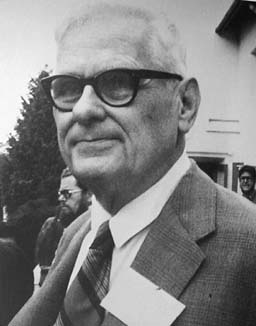
\includegraphics[width=2cm]{./church.jpg}
    \end{tabular}
\end{frame}

\begin{frame}
    \frametitle{Introducci\'on}
    \begin{itemize}
        \item{Una lambda no es nada m\'as y nada menos que una funci\'on.}
        \item{Tradicionalmente, los lenguajes siempre han separado las funciones
        y los valores (eg. metodos y propiedades)}
        \item{Los lambdas permiten utilizar funciones como si fueran valores}
        \item{Esto significa que una funci\'on puede almacenarce en una variable
        o puede pasarse como parametro a un metodo.}
        \item{La brecha entre funciones y valores se rompe al tener un lenguaje
        con lambdas.}
        \item{De hecho, un lenguaje de programaci\'on puede consistir solamente de
        lambdas, el resto son vanidades. El lenguaje Haskell\cite{Haskell}, se apega mucho
        a esta filosofia.}
    \end{itemize}
\end{frame}

\begin{frame}
    \frametitle{Definici\'on de Lambdas}
    El formato para definir lambdas en C\# es: $(\mathtt{arg_1},\ldots,\mathtt{arg_n}) \Rightarrow \{[cuerpo]\}$
    en donde:
    \begin{itemize}
        \item{$\mathtt{arg_1},\ldots,\mathtt{arg_n}$ son variables correspondientes a los
        parametros de la funci\'on.}
        \item{$[cuerpo]$ el el codigo que ejecuta la funcion.}
    \end{itemize}
    {\bf Observaciones: }
    \begin{itemize}
        \item{Es permitido omitir los parentesis de los parametros cuando la funci\'on
        solamente tiene un parametro.}
        \item{Es permitido omitir los corchetes ({}) que rodean el cuerpo de la funci\'on
        si dicho cuerpo solo tiene una linea.}
    \end{itemize}
\end{frame}

\begin{frame}
    \frametitle{La clase \emph{Func}}
    \begin{itemize}
        \item{La clase \emph{Func} se utiliza para definir variables de
        tipo \emph{Funcion} (ie. lambdas)}
        \item{Hay varias definiciones de esta clase, seg\'un la cantidad
        de parametros y el tipo de retorno.}
        \item{Se utiliza de la siguiente manera: $\mathtt{Func}\langle\mathtt{Arg_1},\ldots\mathtt{Arg_n},\mathtt{Res}\rangle$
        donde $\mathtt{Arg_1},\ldots,\mathtt{Arg_n}$ corresponden a los parametros de la funci\'on
        y $\mathtt{Res}$ al resultado de la funci\'on.}
        \item{Por ejemplo, una funci\'on que suma dos numeros enteros, se declararia
        como ``$\mathtt{Func}\langle\mathtt{int},\mathtt{int}\rangle\ sumar$''}
        \item{Ver el metodo \emph{Ejemplo\_Func} del archivo \href{run:../Ejemplos/Lambdas/Program.cs}{Program.cs}}
    \end{itemize}
\end{frame}

\begin{frame}
    \frametitle{La clase \emph{Action}}
    \begin{itemize}
        \item{Tiene la misma funcionalidad basica que \emph{Func}}
        \item{Difiere que se utiliza exculsivamente para funciones \emph{impuras}.}
        \item{Esto quiere decier que no tiene tipo de retorno}
        \item{Por lo cual su utilizaci\'on es: ``$\mathtt{Action}\langle\mathtt{Arg_1},\ldots,\mathtt{Arg_n}\rangle$''
        en donde ``$\mathtt{Arg_1},\ldots,\mathtt{Arg_n}$'' son los tipos de los parametros.}
        \item{Su cuerpo no necesita tener un $\mathtt{return}$ (aunque si lo puede tener.)}
    \end{itemize}
\end{frame}

\begin{frame}
    \frametitle{Funciones de orden superior}
    \begin{itemize}
        \item{Ya vimos que es posible utilizar funciones como valores,
        asignarlos a variables, incluso colocarlos en arreglos!}
        \item{No debe ser extra\~no que tamb\'en pueden ser pasadas como
        parametros a otras funciones o metodos.}
        \item{M\'etodos y funciones que aceptan funciones en sus parametros
        se conocen como \emph{funciones de orden superior}}.
        \item{Ver las funciones \emph{Buscar}, \emph{MaxBy} y \emph{Filtrar}
        que se encuentran en el archivo \href{run:../Ejemplos/Lambdas/Program.cs}{Program.cs}}
    \end{itemize}
\end{frame}

\begin{frame}
    \frametitle{Referencias}
    \bibliography{../../Referencias/referencias}
    \bibliographystyle{plain}
\end{frame}

\end{document}